
%% bare_conf.tex
%% V1.4b
%% 2015/08/26
%% by Michael Shell
%% See:
%% http://www.michaelshell.org/
%% for current contact information.
%%
%% This is a skeleton file demonstrating the use of IEEEtran.cls
%% (requires IEEEtran.cls version 1.8b or later) with an IEEE
%% conference paper.
%%
%% Support sites:
%% http://www.michaelshell.org/tex/ieeetran/
%% http://www.ctan.org/pkg/ieeetran
%% and
%% http://www.ieee.org/

%%*************************************************************************
%% Legal Notice:
%% This code is offered as-is without any warranty either expressed or
%% implied; without even the implied warranty of MERCHANTABILITY or
%% FITNESS FOR A PARTICULAR PURPOSE! 
%% User assumes all risk.
%% In no event shall the IEEE or any contributor to this code be liable for
%% any damages or losses, including, but not limited to, incidental,
%% consequential, or any other damages, resulting from the use or misuse
%% of any information contained here.
%%
%% All comments are the opinions of their respective authors and are not
%% necessarily endorsed by the IEEE.
%%
%% This work is distributed under the LaTeX Project Public License (LPPL)
%% ( http://www.latex-project.org/ ) version 1.3, and may be freely used,
%% distributed and modified. A copy of the LPPL, version 1.3, is included
%% in the base LaTeX documentation of all distributions of LaTeX released
%% 2003/12/01 or later.
%% Retain all contribution notices and credits.
%% ** Modified files should be clearly indicated as such, including  **
%% ** renaming them and changing author support contact information. **
%%*************************************************************************


% *** Authors should verify (and, if needed, correct) their LaTeX system  ***
% *** with the testflow diagnostic prior to trusting their LaTeX platform ***
% *** with production work. The IEEE's font choices and paper sizes can   ***
% *** trigger bugs that do not appear when using other class files.       ***                          ***
% The testflow support page is at:
% http://www.michaelshell.org/tex/testflow/



\documentclass[conference]{IEEEtran}
% Some Computer Society conferences also require the compsoc mode option,
% but others use the standard conference format.
%
% If IEEEtran.cls has not been installed into the LaTeX system files,
% manually specify the path to it like:
% \documentclass[conference]{../sty/IEEEtran}


\usepackage{cite}
\usepackage{amsmath,amssymb,amsfonts}
\usepackage{algorithmic}
\usepackage{graphicx}
\usepackage{textcomp}
\usepackage{xcolor}

\usepackage{pgfplots} % per a graficar amb LaTeX
\pgfplotsset{samples=2000} % número màxim de punts d'una corba que genera ell, canviar
\pgfplotsset{compat=1.16} % perquè si no el pgfplot dóna error
\usepackage{import} % per a les imatges d'Inkscape
\usepackage{xifthen} % per a les imatges d'Inkscape
\usepackage{pdfpages} % per a les imatges d'Inkscape
\usepackage{transparent} % per a les imatges d'Inkscape
\usepackage[RPvoltages]{circuitikz} % per tal que no salti warning
\usetikzlibrary{arrows, decorations.markings, arrows.meta} % per a dibuixar fletxes d'intensitat
\usepackage{gensymb}
\usepackage{steinmetz}


% Some very useful LaTeX packages include:
% (uncomment the ones you want to load)


% *** MISC UTILITY PACKAGES ***
%
%\usepackage{ifpdf}
% Heiko Oberdiek's ifpdf.sty is very useful if you need conditional
% compilation based on whether the output is pdf or dvi.
% usage:
% \ifpdf
%   % pdf code
% \else
%   % dvi code
% \fi
% The latest version of ifpdf.sty can be obtained from:
% http://www.ctan.org/pkg/ifpdf
% Also, note that IEEEtran.cls V1.7 and later provides a builtin
% \ifCLASSINFOpdf conditional that works the same way.
% When switching from latex to pdflatex and vice-versa, the compiler may
% have to be run twice to clear warning/error messages.






% *** CITATION PACKAGES ***
%
%\usepackage{cite}
% cite.sty was written by Donald Arseneau
% V1.6 and later of IEEEtran pre-defines the format of the cite.sty package
% \cite{} output to follow that of the IEEE. Loading the cite package will
% result in citation numbers being automatically sorted and properly
% "compressed/ranged". e.g., [1], [9], [2], [7], [5], [6] without using
% cite.sty will become [1], [2], [5]--[7], [9] using cite.sty. cite.sty's
% \cite will automatically add leading space, if needed. Use cite.sty's
% noadjust option (cite.sty V3.8 and later) if you want to turn this off
% such as if a citation ever needs to be enclosed in parenthesis.
% cite.sty is already installed on most LaTeX systems. Be sure and use
% version 5.0 (2009-03-20) and later if using hyperref.sty.
% The latest version can be obtained at:
% http://www.ctan.org/pkg/cite
% The documentation is contained in the cite.sty file itself.






% *** GRAPHICS RELATED PACKAGES ***
%
\ifCLASSINFOpdf
  % \usepackage[pdftex]{graphicx}
  % declare the path(s) where your graphic files are
  % \graphicspath{{../pdf/}{../jpeg/}}
  % and their extensions so you won't have to specify these with
  % every instance of \includegraphics
  % \DeclareGraphicsExtensions{.pdf,.jpeg,.png}
\else
  % or other class option (dvipsone, dvipdf, if not using dvips). graphicx
  % will default to the driver specified in the system graphics.cfg if no
  % driver is specified.
  % \usepackage[dvips]{graphicx}
  % declare the path(s) where your graphic files are
  % \graphicspath{{../eps/}}
  % and their extensions so you won't have to specify these with
  % every instance of \includegraphics
  % \DeclareGraphicsExtensions{.eps}
\fi
% graphicx was written by David Carlisle and Sebastian Rahtz. It is
% required if you want graphics, photos, etc. graphicx.sty is already
% installed on most LaTeX systems. The latest version and documentation
% can be obtained at: 
% http://www.ctan.org/pkg/graphicx
% Another good source of documentation is "Using Imported Graphics in
% LaTeX2e" by Keith Reckdahl which can be found at:
% http://www.ctan.org/pkg/epslatex
%
% latex, and pdflatex in dvi mode, support graphics in encapsulated
% postscript (.eps) format. pdflatex in pdf mode supports graphics
% in .pdf, .jpeg, .png and .mps (metapost) formats. Users should ensure
% that all non-photo figures use a vector format (.eps, .pdf, .mps) and
% not a bitmapped formats (.jpeg, .png). The IEEE frowns on bitmapped formats
% which can result in "jaggedy"/blurry rendering of lines and letters as
% well as large increases in file sizes.
%
% You can find documentation about the pdfTeX application at:
% http://www.tug.org/applications/pdftex





% *** MATH PACKAGES ***
%
%\usepackage{amsmath}
% A popular package from the American Mathematical Society that provides
% many useful and powerful commands for dealing with mathematics.
%
% Note that the amsmath package sets \interdisplaylinepenalty to 10000
% thus preventing page breaks from occurring within multiline equations. Use:
%\interdisplaylinepenalty=2500
% after loading amsmath to restore such page breaks as IEEEtran.cls normally
% does. amsmath.sty is already installed on most LaTeX systems. The latest
% version and documentation can be obtained at:
% http://www.ctan.org/pkg/amsmath





% *** SPECIALIZED LIST PACKAGES ***
%
%\usepackage{algorithmic}
% algorithmic.sty was written by Peter Williams and Rogerio Brito.
% This package provides an algorithmic environment fo describing algorithms.
% You can use the algorithmic environment in-text or within a figure
% environment to provide for a floating algorithm. Do NOT use the algorithm
% floating environment provided by algorithm.sty (by the same authors) or
% algorithm2e.sty (by Christophe Fiorio) as the IEEE does not use dedicated
% algorithm float types and packages that provide these will not provide
% correct IEEE style captions. The latest version and documentation of
% algorithmic.sty can be obtained at:
% http://www.ctan.org/pkg/algorithms
% Also of interest may be the (relatively newer and more customizable)
% algorithmicx.sty package by Szasz Janos:
% http://www.ctan.org/pkg/algorithmicx




% *** ALIGNMENT PACKAGES ***
%
%\usepackage{array}
% Frank Mittelbach's and David Carlisle's array.sty patches and improves
% the standard LaTeX2e array and tabular environments to provide better
% appearance and additional user controls. As the default LaTeX2e table
% generation code is lacking to the point of almost being broken with
% respect to the quality of the end results, all users are strongly
% advised to use an enhanced (at the very least that provided by array.sty)
% set of table tools. array.sty is already installed on most systems. The
% latest version and documentation can be obtained at:
% http://www.ctan.org/pkg/array


% IEEEtran contains the IEEEeqnarray family of commands that can be used to
% generate multiline equations as well as matrices, tables, etc., of high
% quality.




% *** SUBFIGURE PACKAGES ***
%\ifCLASSOPTIONcompsoc
%  \usepackage[caption=false,font=normalsize,labelfont=sf,textfont=sf]{subfig}
%\else
%  \usepackage[caption=false,font=footnotesize]{subfig}
%\fi
% subfig.sty, written by Steven Douglas Cochran, is the modern replacement
% for subfigure.sty, the latter of which is no longer maintained and is
% incompatible with some LaTeX packages including fixltx2e. However,
% subfig.sty requires and automatically loads Axel Sommerfeldt's caption.sty
% which will override IEEEtran.cls' handling of captions and this will result
% in non-IEEE style figure/table captions. To prevent this problem, be sure
% and invoke subfig.sty's "caption=false" package option (available since
% subfig.sty version 1.3, 2005/06/28) as this is will preserve IEEEtran.cls
% handling of captions.
% Note that the Computer Society format requires a larger sans serif font
% than the serif footnote size font used in traditional IEEE formatting
% and thus the need to invoke different subfig.sty package options depending
% on whether compsoc mode has been enabled.
%
% The latest version and documentation of subfig.sty can be obtained at:
% http://www.ctan.org/pkg/subfig




% *** FLOAT PACKAGES ***
%
%\usepackage{fixltx2e}
% fixltx2e, the successor to the earlier fix2col.sty, was written by
% Frank Mittelbach and David Carlisle. This package corrects a few problems
% in the LaTeX2e kernel, the most notable of which is that in current
% LaTeX2e releases, the ordering of single and double column floats is not
% guaranteed to be preserved. Thus, an unpatched LaTeX2e can allow a
% single column figure to be placed prior to an earlier double column
% figure.
% Be aware that LaTeX2e kernels dated 2015 and later have fixltx2e.sty's
% corrections already built into the system in which case a warning will
% be issued if an attempt is made to load fixltx2e.sty as it is no longer
% needed.
% The latest version and documentation can be found at:
% http://www.ctan.org/pkg/fixltx2e


%\usepackage{stfloats}
% stfloats.sty was written by Sigitas Tolusis. This package gives LaTeX2e
% the ability to do double column floats at the bottom of the page as well
% as the top. (e.g., "\begin{figure*}[!b]" is not normally possible in
% LaTeX2e). It also provides a command:
%\fnbelowfloat
% to enable the placement of footnotes below bottom floats (the standard
% LaTeX2e kernel puts them above bottom floats). This is an invasive package
% which rewrites many portions of the LaTeX2e float routines. It may not work
% with other packages that modify the LaTeX2e float routines. The latest
% version and documentation can be obtained at:
% http://www.ctan.org/pkg/stfloats
% Do not use the stfloats baselinefloat ability as the IEEE does not allow
% \baselineskip to stretch. Authors submitting work to the IEEE should note
% that the IEEE rarely uses double column equations and that authors should try
% to avoid such use. Do not be tempted to use the cuted.sty or midfloat.sty
% packages (also by Sigitas Tolusis) as the IEEE does not format its papers in
% such ways.
% Do not attempt to use stfloats with fixltx2e as they are incompatible.
% Instead, use Morten Hogholm'a dblfloatfix which combines the features
% of both fixltx2e and stfloats:
%
% \usepackage{dblfloatfix}
% The latest version can be found at:
% http://www.ctan.org/pkg/dblfloatfix




% *** PDF, URL AND HYPERLINK PACKAGES ***
%
%\usepackage{url}
% url.sty was written by Donald Arseneau. It provides better support for
% handling and breaking URLs. url.sty is already installed on most LaTeX
% systems. The latest version and documentation can be obtained at:
% http://www.ctan.org/pkg/url
% Basically, \url{my_url_here}.




% *** Do not adjust lengths that control margins, column widths, etc. ***
% *** Do not use packages that alter fonts (such as pslatex).         ***
% There should be no need to do such things with IEEEtran.cls V1.6 and later.
% (Unless specifically asked to do so by the journal or conference you plan
% to submit to, of course. )


% correct bad hyphenation here
\hyphenation{op-tical net-works semi-conduc-tor}


\begin{document}
%
% paper title
% Titles are generally capitalized except for words such as a, an, and, as,
% at, but, by, for, in, nor, of, on, or, the, to and up, which are usually
% not capitalized unless they are the first or last word of the title.
% Linebreaks \\ can be used within to get better formatting as desired.
% Do not put math or special symbols in the title.
\title{Solution to the AC/DC Power Flow with the Holomorphic Embedding Method}


% author names and affiliations
% use a multiple column layout for up to three different
% affiliations
\author{\IEEEauthorblockN{Josep Fanals Batllori}
\IEEEauthorblockA{u1946589@campus.udg.edu}}


% conference papers do not typically use \thanks and this command
% is locked out in conference mode. If really needed, such as for
% the acknowledgment of grants, issue a \IEEEoverridecommandlockouts
% after \documentclass

% for over three affiliations, or if they all won't fit within the width
% of the page, use this alternative format:
% 
%\author{\IEEEauthorblockN{Michael Shell\IEEEauthorrefmark{1},
%Homer Simpson\IEEEauthorrefmark{2},
%James Kirk\IEEEauthorrefmark{3}, 
%Montgomery Scott\IEEEauthorrefmark{3} and
%Eldon Tyrell\IEEEauthorrefmark{4}}
%\IEEEauthorblockA{\IEEEauthorrefmark{1}School of Electrical and Computer Engineering\\
%Georgia Institute of Technology,
%Atlanta, Georgia 30332--0250\\ Email: see http://www.michaelshell.org/contact.html}
%\IEEEauthorblockA{\IEEEauthorrefmark{2}Twentieth Century Fox, Springfield, USA\\
%Email: homer@thesimpsons.com}
%\IEEEauthorblockA{\IEEEauthorrefmark{3}Starfleet Academy, San Francisco, California 96678-2391\\
%Telephone: (800) 555--1212, Fax: (888) 555--1212}
%\IEEEauthorblockA{\IEEEauthorrefmark{4}Tyrell Inc., 123 Replicant Street, Los Angeles, California 90210--4321}}




% use for special paper notices
%\IEEEspecialpapernotice{(Invited Paper)}




% make the title area
\maketitle

% As a general rule, do not put math, special symbols or citations
% in the abstract
\begin{abstract}
The Holomorphic Embedding Load-Flow Method has been regarded as a powerful and complete tool to solve to AC power flow. Its theoretical base makes it stand apart from the traditional iterative methods, which suffer from convergence issues and are not guaranteed to obtain a feasible solution. 

The application of the holomorphic embedding method to the DC power flow as well as circuits with nonlinear devices has been very limited. Despite that, its properties are meant to still be favorable. Some technologies have been growing in popularity, like DC power systems, which are regarded as less costly than AC power systems for large distances. 

This paper approaches the solution to the AC/DC power flow by means of the holomorphic embedding method. A simplistic test case is considered in order to show the performance of the algorithm. 
\end{abstract}
\begin{IEEEkeywords}
power flow, holomorphic embedding, AC/DC, convergence, rectifier, inverter
\end{IEEEkeywords}  

% no keywords




% For peer review papers, you can put extra information on the cover
% page as needed:
% \ifCLASSOPTIONpeerreview
% \begin{center} \bfseries EDICS Category: 3-BBND \end{center}
% \fi
%
% For peerreview papers, this IEEEtran command inserts a page break and
% creates the second title. It will be ignored for other modes.
\IEEEpeerreviewmaketitle

\section{Introduction}\label{secIntro}
It is a well-known fact that the equations that define the load flow of electric power systems are nonlinear. Since they can not be solved directly through a linear system of equations, iterative methods have been to go-to option \cite{Gomez}. Among them, the Newton-Rapshon has been the most popularized choice, since it usually converges with few iterations. 

By definition, ill-conditioned systems operate under conditions that increase the difficulty to solve them. Two problems arise with iterative algorithms: first, the method may diverge even though there is a feasible solution, and in second place, the method could converge to a mathematically possible but physically infeasible result \cite{Tripathy}.

In contrast, the holomorphic embedding method consists in a recursive algorithm that builds the solution step by step. It is based on complex analysis, algebraic curves and approximation theory \cite{Trias2018}. Its major upside is that it can tell when the solution is infeasible and find out the result when the power flow is feasible.

HVDC systems have been proven to be a reliable and cost-saving choice \cite{Arrillaga1993} with increasing popularity \cite{Kothari}. The interconnection between the AC and the DC system is due to a converter, which acts as a rectifier or an inverter. Its equations are nonlinear. Thus, several works have employed the Newton-Raphson method to solve them \cite{Arrillaga1978}, \cite{Arrillaga1993}, \cite{Arrillaga1994} and \cite{Arrillaga2002}.

This paper focuses on formulating the equations that define the AC/DC converter in a way that makes them solvable with the holomorphic embedding. A basic system has been selected to show the derivation of the equations. More complex systems could also be solved by following a similar procedure. One of its advantages is found in that the typical AC formulation could add without much complexity the presence of the AC/DC converter. Furthermore, Sigma approximants, which are used as a diagnostic tool \cite{Trias2018}, would remain valid for the AC side.

The paper is structured as follows: Section \ref{equacions} presents the simple test case and its equations; Section \ref{incrust} adapts the equations to the holomorphic embedding method; Section \ref{algoritme} details the algorithm to be followed at each step of the process; Section \ref{resultats} shows the most interesting results that have been generated; finally, Section \ref{secConcl} concludes the paper and mentions what the future work could be. 

\section{AC/DC systems equations}\label{equacions}
AC/DC converters station consists of a structure that contains a transformer used to adjust voltages as well as a converter. That last item is the main responsible of the transformation from AC to DC or vice-versa. In the first case, it would act as a rectifier, while in the second, as an inverter. Its functionality can be reversed since it can be understood as a three-phase bridge with thyristors. The behavior is dependent upon the chosen delay angle for the thyristors. If the delay angle $0<\alpha<90^{\circ}$ it operates as a rectifier; if $180^{\circ}>\alpha>90^{\circ}$ it acts as an inverter.

The aforementioned stations could also incorporate filters, reactive power compensators, a smoothing reactor, etc. All these auxiliary components do not play a critical role during the fundamental analysis of the converter, so they will be omitted. 

A simple system such as the one in Figure \ref{fig:sistema} will be employed to present the equations involved and the corresponding embedding. It has already been converted to a per-unit base system. The transformer stands as an off-nominal transformer due to the fact that base voltages may not match their nominal voltages.
\begin{figure}[!htb]
  \begin{center}
  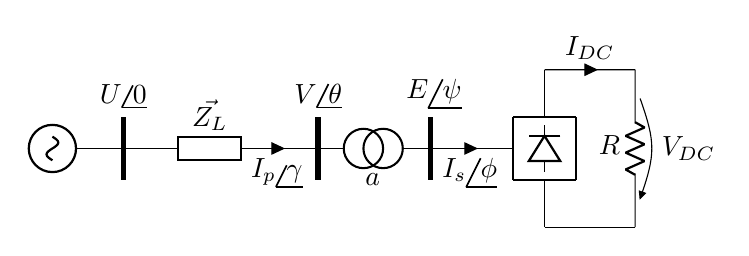
\begin{tikzpicture}[scale = 1, transform shape]
    \draw (0, 0) to [/tikz/circuitikz/bipoles/length=1.0cm, sV] (0.6, 0);
    \ctikzset{resistor = european}
    \draw (0.6, 0) to [/tikz/circuitikz/bipoles/length=1.0cm, resistor] (4, 0);
    \draw [line width=0.75] (4.25, 0) circle (0.25);
    \draw [line width=0.75] (4.5, 0) circle (0.25);
    \draw (4.75, 0) to [short] (5.2, 0);
    \draw (5.2, 0) to [short, i_=$I_s\phase{\phi}$] (6.0, 0);
    \draw (6.0, 0) to [short] (6.15, 0);
    \draw (6.15+0.4, -0.3) to [/tikz/circuitikz/bipoles/length=0.8cm, empty diode] (6.15+0.4, 0.3);
    \draw [line width=0.75] (6.15, -0.4) -- (6.15, 0.4);
    \draw [line width=0.75] (6.95, -0.4) -- (6.95, 0.4);
    \draw [line width=0.75] (6.15, -0.4) -- (6.95, -0.4);
    \draw [line width=0.75] (6.15, 0.4) -- (6.95, 0.4);
    \draw (6.55, 0.4) -- (6.55, 1.0);
    \draw (6.55, -0.4) -- (6.55, -1.0);
    \draw (6.55, 1.0) to [short, i=$I_{DC}$] (7.7, 1.0);
    \draw (6.55, -1.0) -- (7.7, -1.0);
    \ctikzset{resistor = american}
    \draw (7.7, -1.0) to [/tikz/circuitikz/bipoles/length=0.8cm, resistor, l=$R$,v_=$V_{DC}$] (7.7, 1.0);
    \draw [line width=2] (1.2, -0.4) -- (1.2, 0.4);
    \draw [line width=2] (3.675, -0.4) -- (3.675, 0.4);
    \draw [line width=2] (5.1, -0.4) -- (5.1, 0.4);
    \draw (4.67, 0.51) node[anchor=south west] {$E\phase{\psi}$};
    \draw (3.25, 0.45) node[anchor=south west] {$V\phase{\theta}$};
    \draw (0.78, 0.45) node[anchor=south west] {$U\phase{0}$};
    \draw (1.95, 0.1) node[anchor=south west] {$\vec{Z_L}$};
    \draw (2.9, 0) to [short, i_=$I_p\phase{\gamma}$] (3.4, 0);
    \draw (4.15, -0.60) node[anchor=south west] {$a$};
  \end{tikzpicture}
  \caption{Simplified system with an AC/DC converter}
  \label{fig:sistema}
  \end{center}
  \end{figure}

The combination of AC and DC power flow has traditionally implied a decoupling of references between both types of systems \cite{Arrillaga1978}, \cite{Arrillaga2002}. On the one hand, the DC power flow sets the reference to $I_s$, while the AC power flow establishes it to the slack bus voltage. A side-effect of that is that even though the absolute value of the variable $V$ remains the same, its phase change according to the chosen system, either the AC or DC part.

Despite not being mandatory to set $I_s\phase{0}$, it is regarded as a convenient option \cite{Arrillaga1994}. Note that $I_p$ coincides in phase to $I_s$ because the transformer is assumed to be ideal. There is no leakage reactance to take into account, only the off-nominal tap ratio $a$. However, the derivation of equations will consider the reference chosen in Figure \ref{fig:sistema}, i.e. the systems will not be decoupled when solved with the holomorphic embedding method, the reason being that it becomes much more complex when embedding angles.

The equations that define the DC power flow in a given per unit base system \cite{Arrillaga1994} are
\begin{equation}
  \begin{cases}
V_{DC}=&k_1aV\cos\alpha - 3\frac{X_c}{\pi}I_{DC},\\
P_{DC}=&\Re[V\phase{\theta}I_p\phase{\gamma}],\\
V_{DC}=&I_{DC}R,\\
  \end{cases}
    \label{eq:1}
  \end{equation}
where $X_c$ is the commutation reactance, $P_{DC}$ the power demand at the DC side, $\alpha$ the delay angle and $k_1=\frac{3\sqrt{2}}{\pi}$. The commutation overlap, which would slightly modify $k_1$ will be ignored, but it could be considered without further consequences \cite{Arrillaga1994}. 

On the AC side, the first KCL has to be evaluated in order to find the expression that must equal $I_p\phase{\gamma}$. Two equations will be derived from that: one for the real part and the other concerning the imaginary part. First, it should be noted that
\begin{equation}
  I_p=k_1aI_{DC},
  \label{eq:2}
\end{equation}
so $I_p$ will no longer be treated directly as an unknown \cite{Arrillaga1978}, \cite{Arrillaga1993} and \cite{Arrillaga1994}. Both $a$ and $I_{DC}$ will have to be found. The balance of currents yields 
\begin{equation}
  \begin{cases}
   \Re[I_p\phase{\gamma}]&=UG-VG\cos\theta+VB\sin\theta,\\
   \Im[I_p\phase{\gamma}]&=UB-VG\sin\theta-VB\cos\theta, \\
  \end{cases}
  \label{eq:3}
\end{equation}
where $G$ and $B$ represent the real and imaginary part of $1/\vec{Z_L}$.

At that stage of the formulation, there are five relevant equations and a total of seven variables ($V$, $\theta$, $\gamma$, $V_{DC}$, $I_{DC}$, $a$ and $\cos\alpha$). Two control equations have to be added for each converter \cite{Arrillaga1994}. Out of a handful of expressions to choose, the selected ones become
\begin{equation}
  \begin{cases}
   a^{sp}&=a,\\
  P^{sp}_{DC}&=V_{DC}I_{DC},\\ 
  \end{cases}
  \label{eq:4}
\end{equation}
where $a^{sp}$ is the specified off-nominal tap ratio and $P^{sp}_{DC}$ corresponds to the specified DC power. In reality, they would depend on the desired operative state. For convenience, in that example it developed from an arbitrary choice. 

Since the DC power is known and also the resistive load, $V_{DC}$ and $I_{DC}$ can be found without any other information. Furthermore, because $a$ turns out not to be a variable, from a total of seven variables, four of them have to be calculated ($V$, $\theta$, $\gamma$, $\cos\alpha$). 

\section{Embedding}\label{incrust}
The Holomorphic Embedding Method has been proven to also be a fertile ground of development for DC circuits with nonlinear loads, for instance \cite{Trias2016}. Just like the AC power flow, the first step consists in embedding the equations. Then, the first coefficients have to be obtained so that the reference state becomes fully defined. From then on the solution is built by calculating more and more coefficients. 

The choice of embedding is not unique \cite{Trias2018}. In the AC power flow there have been some variations that embed the equations differently \cite{Wallace} and \cite{Chiang} from the most notorious source, which is \cite{Trias2018}. When it comes to the DC power flow, the selection is probably even more diverse, due to containing several elements and not possessing a reference like the slack bus. 

In the example, first of all, it is interesting to define $V\phase{\theta}$ as
\begin{equation}
  V\phase{\theta}=V^{re}+jV^{im},
  \label{eq:5}
\end{equation}
Right now they are not embedded, but they will eventually become dependent on the complex variable $s$. Let $C$ be a generic variable. When it is embedded, it becomes $C(s)$, which in turn, follows
\begin{equation}
  C(s)=\sum_{k=0}^{n}s^kC[k],
  \label{eq:serie}
\end{equation}
where $C[k]$ represents one term that along with many others conform $C(s)$ and $n$ symbolizes the arbitrary maximum index. Consequently, $C(s)$ contains $n+1$ terms. 

Given that $I_p\phase{\gamma}$ has been divided between real and imaginary part, it ought to be treated as such in \eqref{eq:1}. As a result of that along with the chosen embedding, the second expression of \eqref{eq:1} transforms into
\begin{equation}
  \begin{split}
  sP_{DC}=&GU(s)V^{re}(s)-GV^{re}(s)V^{re}(s)\\
  &+BU(s)V^{im}(s)-GV^{im}(s)V^{im}(s).
  \end{split}
  \label{eq:mod1}
\end{equation}
The proposed embedding is adequate to force the initialization $V^{re}[0]=1$, $V^{im}[0]=0$. That harmonizes with the reference state described in \cite{Trias2018}. To achieve that without invalidating the equations, the slack bus is embedded as
\begin{equation}
  U(s)=1+s(U_w-1),
  \label{eq:slack_emb}
\end{equation}
where $U_w$ is the data of the voltage corresponding to the slack bus. 

There are two remaining equations to embed. One comes from the first expression in \eqref{eq:1}. Postulating the equality of absolute values, it turns out to be
\begin{equation}
  \begin{split}
  \left(\frac{V_{DC}}{k_1a} + \frac{3X_cI_{DC}}{\pi k_1a}\right)^2=&V^{re}(s)V^{re}(s)\alpha(s)\alpha(s) \\
  &+ V^{im}(s)V^{im}(s)\alpha(s)\alpha(s),
  \end{split}
  \label{eq:abs2}
\end{equation}
where $\alpha(s)$ represents $\cos\alpha(s)$.
A concern could emerge from \eqref{eq:abs2}: the product of series at the right hand-side would imply a convolution of four series. That is unusual since the AC power flow is solved with only convolutions of two series \cite{Rao} and \cite{Trias2018}. Nevertheless, that triple convolution will prove to be a solid choice. 

The last equation needed to be incorporated is the one that integrates the definition of $I_p$ seen from the DC side and the one the AC side of the system. By establishing the equality of absolute values
\begin{equation}
  \begin{split}
  s\frac{(ak_1I_{DC})^2}{Y^2} &- U(s)U(s)=V^{re}(s)V^{re}(s)\\
  &+V^{im}(s)V^{im}(s)-s2U(s)V^{re}(s),
  \end{split}
  \label{eq:abs3}
\end{equation}
where $Y^2=G^2+B^2$. In both \eqref{eq:mod1} and \eqref{eq:abs3} there are some terms that multiply directly by $s$ and as a consequence of that their usage is delayed. The purpose behind that lies in conditioning the system of equations so that they remain consistent with the reference state as well as not blocking the access to the solutions. For instance, if the delay of $P_{DC}$ in \eqref{eq:mod1} did not take place, the reference state would be invalidated; on the other hand, multiplying $U(s)V^{re}(s)$ by $s$ is required in order to formulate a determined system of equations.

Once all the equations are properly embedded, the next process is concerned in calculating the terms that build the series. Once the series are constructed, the last step to find the final solution evaluates the series at $s=1$. That can be achieved thanks to Padé approximants with great precision \cite{Trias2018}. They are not the only tool available. Recursive approaches like Wynn's $\epsilon$ or Bauer's $\eta$ could also be employed \cite{Rao}, and even the sum of coefficients is a suitable alternative if the radius of convergence is bigger than the unit.
% --------------

% As a result of \eqref{eq:5}, from \eqref{eq:1}, the real part of $V$ becomes a known value by means of
% \begin{equation}
%   V^{re}=\frac{V_{DC}}{k_1a}.
%   \label{eq:6}
% \end{equation}
% Since that part has already been found, there is no point in embedding it. Therefore, \eqref{eq:5} is embedded as
% \begin{equation}
%   \begin{cases}
%   |V(s)||V(s)|&=V^{re}V^{re}+sV^{im}(s)V^{im}(s) + (1-s)V_0,\\  
%   UU&=U^{re}(s)U^{re}(s)+U^{im}(s)U^{im}(s).\\
%   \end{cases}
%   \label{eq:7}
% \end{equation}
% It is beneficial to work with the absolute value of $V(s)$ because that is the one that appears in the first expression of \eqref{eq:1}. The addition of $V_0$ may not be strictly required, but it is advised in order to initialize $|V(s)|$ to an appropriate value.  

% Considering \eqref{eq:5}, a possible embedding for \eqref{eq:3} becomes
% \begin{equation}
%   \begin{cases}
%     ak_1I_{DC}&=U^{re}(s)G-sU^{im}(s)B-V^{re}(s)G\\
%     &+sV^{im}(s)B,\\
%    0&=sU^{im}(s)G+U^{re}(s)B-V^{im}(s)G\\
%    &-V^{re}(s)B, \\
%   \end{cases}
%   \label{eq:8}
% \end{equation}
% The effect of multiplying by $s$ implies that a given variable will be ignored while calculating the reference state (terms of the form $[0]$). Thus, it facilitates the initialization. The remaining equation to embed transforms into
% \begin{equation}
%   |V(s)|\cos\alpha(s)=\frac{V_{DC}}{k_1a}+\frac{3X_cI_{DC}}{\pi k_1a}.
%   \label{eq:9}
% \end{equation}
% The goal in mind with that embedding is to be able to formulate a recursive algorithm where no system of equations is involved. The method still works with a linear system of equations at each step (the AC power flow is based on that), although the algorithm gains simplicity by avoiding it. 

% Once all the equations are properly embedded, the next process is concerned in calculating the terms that build the series. When the series are constructed, the last step to find the final solution evaluates the series at $s=1$. That can be achieved thanks to Padé approximants with great precision \cite{Trias2018}. They are not the only tool available. Recursive approaches like Wynn's $\epsilon$ or Bauer's $\eta$ could also be employed \cite{Rao}, and even the sum of coefficients is a suitable alternative if the radius of convergence is bigger than the unit.
\section{Algorithm}\label{algoritme}
The combination of \eqref{eq:mod1}, \eqref{eq:abs2} and \eqref{eq:abs3} must not be straigthforward. At that stage, the unknowns are $V^{re}(s)$, $V^{im}(s)$ and $\alpha(s)$. \eqref{eq:mod1} and \eqref{eq:abs3} do not depend upon $\alpha(s)$, so the coefficients that conform $V^{re}(s)$ and $V^{im}(s)$ must be extracted from these expressions. Then, they have to be employed in \eqref{eq:abs2} to solve for $\alpha(s)$. 

Hence, a two-step process is constructed. The first step builds a system of two equations. Its solution generates a further coefficient of $V^{re}(s)$ and $V^{im}(s)$. Then, this information is used in the triple convolutions that revolve around $\alpha(s)$. Because of that, a new coefficient of $\alpha(s)$ is obtained. 


The algorithm has to be split into the calculation of the terms $[0]$, $[1]$, $[2]$ and $[c\geq 3]$ since it can only be generalized once the first steps are completed. 
As mentioned, $V^{re}[0]=1$ and $V^{im}[0]=0$. On the other hand, it is convenient not to force $\alpha[0]$. Its initial value my be distant from the final result and there is hardly any intuition on what it may become. Thus, using \eqref{eq:abs2} yields
\begin{equation}
  \alpha[0] = \pm\sqrt{\left(\frac{V_{DC}}{k_1a}+\frac{3X_cI_{DC}}{\pi k_1a}\right)^2}.
  \label{eq:alpha0}
\end{equation}
Only the positive root should be selected, as it can be deduced from the original expression captured in \eqref{eq:1}. 

The next step consists in obtaining the first order coefficients. Consequently, a system of equations is formed from \eqref{eq:mod1} and \eqref{eq:abs3}. Fortunately, just like it happens during the AC power flow implementation of the holomorphic embedding, the matrix turns out to be constant at all steps. It becomes an upside in contrast to the Newton-Raphson, where the linear system has to be reconstructed at each iteration. The generalized system comes to be
\begin{equation}
  \begin{pmatrix}
    R1[c]\\
    R2[c]
  \end{pmatrix}
  =
  \begin{pmatrix}
    -G & B \\
    2 & 0
  \end{pmatrix}
  \begin{pmatrix}
    V^{re}[c]\\
    V^{im}[c]
  \end{pmatrix},
  \label{eq:sist1}
\end{equation}
where $R1[c]$ and $R2[c]$ are the right hand-side expressions that have to be computed for every step. For the first order coefficients
\begin{equation}
  \begin{cases}
    R1[1]=&P_{DC}-GV^{re}[0](U-1),\\
    R2[1]=&\frac{ak_1I_{DC}}{Y^2}-2(U-1).\\
  \end{cases}
  \label{eq:r1r21}
\end{equation}
Subsequently, $V^{re}[1]$ and $V^{im}[1]$ become known. The last calculation to perform at this step is
\begin{equation}
  \alpha[1]=-\frac{V^{re}[1]\alpha[0]}{V^{re}[0]}.
  \label{eq:alph1}
\end{equation}
At this stage all the first order cofficients have been obtained. Next, the algorithm is explicitly defined for the $[2]$ terms, and then, generalized. 

The following terms start involving trivial convolutions, which will be more and more prominent at each step. When it comes to the system of equations, the right hand-side expressions are derived as
\begin{equation}
\begin{cases}
  R1[2]=&-GV^{re}[1](U-1)-BV^{im}[1](U-1)\\
  &+G\sum_{k=1}^1V^{re}[k]V^{re}[2-k]\\
  &+G\sum_{k=1}^1V^{im}[k]V^{im}[2-k],\\
  R2[2]=&-(U-1)(U-1)+2V^{re}[1]+2(U-1)\\
  &-\sum_{k=1}^1V^{re}[k]V^{re}[2-k]\\
  &-\sum_{k=1}^1V^{im}[k]V^{im}[2-k].\\
\end{cases}
  \label{eq:r1r22}
\end{equation}
Employing \eqref{eq:sist1} and \eqref{eq:r1r22} provides the desired voltage coefficients. Then, the expression to compute $\alpha[2]$ also increases its complexity, transforming into
\begin{equation}
  \begin{split}
  \alpha[2] =& \biggl(-\sum_{k=1}^1\alpha[k]\alpha[2-k]\\
  &-\sum_{k=1}^2(V^{re})^2[k]\sum_{j=0}^{2-k}\alpha[j]\alpha[2-k-j]\\
  &-\sum_{k=1}^2(V^{im})^2[k]\sum_{j=0}^{2-k}\alpha[j]\alpha[2-k-j]\biggr)\frac{1}{2\alpha[0]},
  \end{split}
  \label{eq:alph2}
\end{equation}
where $(V^{re})^2(s)$ corresponds to the squared $V^{re}(s)$. It must no be confused with squaring a given term. From now on the algorithm can be fully generalized. Given an arbitrary depth $c\geq 3$ the right hand-side expressions that participate in the system of equations turn out to be
\begin{equation}
\begin{cases}
  R1[c]=&-GV^{re}[c-1](U-1)-BV^{im}[c-1](U-1)\\
  &G\sum_{k=1}^{c-1}V^{re}[k]V^{re}[c-k]\\
  &G\sum_{k=1}^{c-1}V^{im}[k]V^{im}[c-k],\\
  R2[c]=&2(U-1)V^{re}[c-2]+2V^{re}[c-1]\\
  &-\sum_{k=1}^{c-1}V^{re}[k]V^{re}[c-k]\\
  &-\sum_{k=1}^{c-1}V^{im}[k]V^{im}[c-k].\\
\end{cases}
  \label{eq:rhsc}
\end{equation}
Finally, the terms that conform $\alpha[c]$ ressemble $\alpha[2]$. In fact, \eqref{eq:alph2} is the particular case of
\begin{equation}
  \begin{split}
  \alpha[c]=& \biggl(-\sum_{k=1}^1\alpha[k]\alpha[c-k]\\
  &-\sum_{k=1}^c(V^{re})^2[k]\sum_{j=0}^{c-k}\alpha[j]\alpha[c-k-j]\\
  &-\sum_{k=1}^c(V^{im})^2[k]\sum_{j=0}^{c-k}\alpha[j]\alpha[c-k-j]\biggr)\frac{1}{2\alpha[0]}.
  \end{split}
  \label{eq:alphc}
\end{equation}
Other embeddings could also be feasible. However, the advantage of opting for the presented one is that it is compatible with the AC power flow, in the sense that voltages are divided in real and imaginary part. Furthermore, $\alpha(s)$ does not intervene in the AC power flow. Accordingly, the AC power flow could be modified to just integrate the bus that connects with the DC system, and then, compute the delay angle $\alpha$ from that. 

Another step further, $alpha$ is obtainable from the final voltage values. So, it is not mandatory to embed it and decompose it with terms to then calculate the resulting value. The reason behind the adopted choice was to show that it is possible to adapt an equation that contains the absolute value of a variable. 

The AC bus that links the AC system with the DC side could interconnect several buses, and not just the slack bus. In that case, the formulation would just need to express the current $I_p$ as a function of voltages and admittances. The same procedure would follow from that, and an algorithm of a similar fashion would be obtained. 

% ----------------------


% \begin{equation}
%   \begin{cases}
%     |V[0]|&=\sqrt{V^{re}V^{re}+V_0},\\
%     \cos\alpha[0]&=\frac{V_{DC}}{k_1a|V[0]|}+\frac{3X_cI_{DC}}{\pi k_1a|V[0]|},\\
%     U^{re}[0]&=\frac{k_1aI_{DC}+GV^{re}}{G},\\
%     V^{im}[0]&=\frac{-BU^{re}[0]+BV^{re}}{-G},\\
%     U^{im}[0]&=\pm\sqrt{U^2-U^{re}[0]U^{re}[0]},\\
%   \end{cases}
%   \label{eq:terms0}
% \end{equation}
% where in the last expression the selection of one sign or the other should not be a critical decision. As \eqref{eq:terms0} manifests, the calculation of a term only depends on already known coefficients.

% The second coefficient of each unknown follows
% \begin{equation}
%   \begin{cases}
%     |V[1]|&=\frac{V^{im}[0]V^{im}[0]-V_0}{2|V[0]|},\\
%     \cos\alpha[1]&=\frac{-|V[1]|\cos\alpha[0]}{|V[0]|},\\
%     U^{re}[1]&=\frac{BU^{im}[0]-BV^{im}[0]}{G},\\
%     V^{im}[1]&=\frac{GU^{im}[0]+BU^{re}[1]}{G},\\
%     U^{im}[1]&=\frac{-U^{re}[0]U^{re}[1]}{U^{im}[0]}.\\
%   \end{cases}
%   \label{eq:terms1}
% \end{equation}
% Again, it is also the case that the new coefficients only depend on the already known terms. Lastly, the algorithm can be generalized for a given depth called $c$
% \begin{equation}
%   \begin{cases}
%     |V[c]|&=\frac{-\sum_{k=1}^{c-1}|V[k]||V[c-k]|+\sum_{k=0}^{c-1}V^{im}[k]V^{im}[c-1-k]}{2|V[0]|},\\
%     \cos\alpha[c]&=\frac{-\sum_{k=0}^{c-1}\cos\alpha[k]|V[c-k]}{|V[0]|},\\
%     U^{re}[c]&=\frac{BU^{im}[c-1]-BV^{im}[c-1]}{G},\\
%     V^{im}[c]&=\frac{GU^{im}[c-1]+BU^{re}[c]}{G},\\
%     U^{im}[c]&=\frac{-\sum_{k=0}^c U^{re}[k]U^{re}[c-k] - \sum_{k=1}^{c-1}U^{im}[k]U^{im}[c-k]}{2U^{im}[0]}.\\
%   \end{cases}
%   \label{eq:terms2}
% \end{equation}
% In contrast to an iterative scheme like the Newton-Raphson method, the derived method does not need to work with a matrix. That alone simplifies the complexity of the algorithm. Even if one does not embed the equations in the same exact way and requires the inversion or factorization of a matrix, it is manageable to obtain a constant matrix. As such, it would not be modified at each step so the runtime would benefit from that. 

\section{Results}\label{resultats}
The covered formulation is applied to a simple system like the one in \ref{fig:sistema}. Table \ref{tab:1} captures the initial data of the problem. All values are expressed per unit according to their respective base.

\begin{table}[!ht]
\renewcommand{\arraystretch}{1.0}
\caption{Data of simple AC/DC system}
\label{tab:1}
\centering
\begin{tabular}{cc}
\hline
Magnitude & Value\\
\hline
$P_{DC}$ & 0.1\\
$R$ & 10\\
$X_c$ & 0.05\\
$U$ & 1.1\\
$a$ & 2\\
$k_1$ & $3\sqrt{2}/\pi$ \\
$G$ & 1\\
$B$ & -1\\
\hline
\end{tabular}
\end{table}

This section focuses on evaluating up to which point the solution given by the holomorphic embedding method remains correct, finding out its convergence properties and discovering the evolution of the error given diverse input values. 

The solution corresponding to the data from Table \ref{tab:1} is shown in Table \ref{tab:2}.
\begin{table}[!ht]
\renewcommand{\arraystretch}{1.0}
\caption{Solution to the simple AC/DC system}
\label{tab:2}
\centering
\begin{tabular}{cc}
\hline
Magnitude & Value\\
\hline
$V^{re}$ & 0.9180\\
$V^{im}$ & 0.0579\\
$\cos\alpha$ & 0.4044\\
\hline
\end{tabular}
\end{table}

At first sight, the results seem coherent. The voltage magnitude is slightly below $U$ since the converter acts as a rectifier, while $\alpha=66.15^{\circ}$. For normal operation the delay angle tends to remain close to $10^{\circ}$ \cite{Kothari}, which is clearly not the case. The values correspond to a made-up case, so there is hardly any logic behind them. The maximum error is 2.1$\cdot 10^{-11}$, sufficiently small. 

To obtain these results, a depth of 60 coefficients has been used. The study of an optimal depth still poses a question without a definite answer. AC power systems are usually solvable with around 20 to 40 coefficients \cite{Rao} and \cite{Trias2018}. Using more coefficients yields a smaller error if the series are convergent enough. When that is not the case, increasing the depth could have tragic effects because the solution could become degraded. Figure \ref{fig:0} plots the maximum error depending on the current depth. 

\begin{figure}[!ht]\footnotesize
\centering
\begin{tikzpicture}
    \begin{axis}[
        /pgf/number format/.cd, ylabel={$\log|$Error$|$},xlabel={Number of coefficients},domain={-0.25:0.25},width=7cm,height=6.5cm,scatter/classes={%
      b={mark=x,mark size=1.0pt,draw=black},c={mark=o,mark size=1.0pt,draw=black}}]]
    \addplot[scatter, scatter src=explicit symbolic]%
        table[x = x, y = y, meta = label, col sep=semicolon] {Resultats/inici2.csv};
        %\legend{, Alternative, Canonical}
    \end{axis}
    \end{tikzpicture}
\caption{Maximum errors depending on the number of coefficients}
\label{fig:0}
\end{figure}

Despite its chaotic nature, the error diminishes quite steadily until it reaches about $10^{-10}$. From then on, the usage of more terms does not improve meaningfully the solution. That pattern of behavior is similar to the ones in the AC power flow \cite{Rao}.  

Under the proposed conditions the series that define by which the unknowns are defined do not converge, yet they slowly diverge. This is not problematic as long as the resulting error turns out to be sufficiently small. By means of Padé approximants one can obtain a solution that converges while the coefficients that conform the series do not. Figure \ref{fig:1} plots the logarithm of the absolute value of the terms corresponding to $V^{re}(s)$. 

\begin{figure}[!ht]\footnotesize
\centering
\begin{tikzpicture}
    \begin{axis}[
        /pgf/number format/.cd, ylabel={$\log|V^{re}[i]|$},xlabel={$i$},domain={-0.25:0.25},width=7cm,height=6.5cm,scatter/classes={%
      b={mark=x,mark size=1.0pt,draw=black},c={mark=o,mark size=1.0pt,draw=black}}]]
    \addplot[scatter, scatter src=explicit symbolic]%
        table[x = x, y = y, meta = label, col sep=semicolon] {Resultats/inici3.csv};
        %\legend{, Alternative, Canonical}
    \end{axis}
    \end{tikzpicture}
\caption{Logarithm of the $V^{re}(s)$ terms to evaluate the convergence}
\label{fig:1}
\end{figure}

From what can be derived, right from the start the coefficients diminish. However, around the fifth coefficient, they start increasing until the plot presents a caveat. From that point on, they keep on increasing. As a result of that, the radius of convergence is smaller than 1, but not distant from it. It is approximately 0.95. 

Hence, the summation of coefficients is not suitable \cite{Trias2018} so some method of analytical continuation must be used, the Padé approximants being the most renowned option. It has been precisely the chosen resource. 

Finally, the evolution of the maximum error as a function of the active power demand at the DC bus is displayed in Figure \ref{fig:2}. 60 coefficients in each series have been used. 
\begin{figure}[!ht]\footnotesize
\centering
\begin{tikzpicture}
    \begin{axis}[
        /pgf/number format/.cd, ylabel={$\log|$Error$|$},xlabel={$P_{DC}$},domain={-0.25:0.25},width=7cm,height=6.5cm,scatter/classes={%
      b={mark=x,mark size=1.0pt,draw=black},c={mark=o,mark size=1.0pt,draw=black}}]]
    \addplot[scatter, scatter src=explicit symbolic]%
        table[x = x, y = y, meta = label, col sep=semicolon] {Resultats/inici4.csv};
        %\legend{, Alternative, Canonical}
    \end{axis}
    \end{tikzpicture}
\caption{Maximum errors depending on $P_{DC}$}
\label{fig:2}
\end{figure}
The error is at its minimum around $P_{DC}=0.1$, which matches the value from Table \ref{tab:1}. Increasing the power implies that the error rises up to a maximum. It then decreases for $P_{DC}\approx 0.4$. From then on, the error keeps more or less constant at around the unit. 

One possible hypothesis for that is found in the fact that $V_{DC}$ and $I_{DC}$ depend on both $P_{DC}$ and $R$. Thus, since $R$ has not changed when $P_{DC}$ is being modified, it is possible that their combination of values causes $V_{DC}$ and $I_{DC}$ to approach values for which the power system analysis is ill-conditioned. 

%posar taula amb números, presentar la solució final i comentar-la. Llavors treure resultats de la convergència de les sèries i així. 

\section{Conclusion}\label{secConcl}
It has been shown that the holomorphic embedding method can also be used to solve the equations involved in the AC/DC power flow with a similar algorithm to the one used for the AC power flow, where rectangular coordinates are also employed. No decoupling of references between systems was needed. Depending on the given control equations the formulation would change, yet the main idea remains the same. 

The performance of the algorithm offers a margin of improvement, since the coefficients do not converge. Other embeddings could be chosen and probably the solution would become more well-conditioned. Despite that, Padé approximants have been useful to find a final convergent solution. Its error decays with the number of iterations. 

The properties of the algorithm remain to be checked for systems with a multitude of buses and converters. It would also be beneficial to compare the holomorphic embedding to the Newton-Raphson in order to find out which one is more convenient under diverse conditions. 



% conference papers do not normally have an appendix


% use section* for acknowledgment
% \section*{Acknowledgment}
% The authors would like to thank...





% trigger a \newpage just before the given reference
% number - used to balance the columns on the last page
% adjust value as needed - may need to be readjusted if
% the document is modified later
%\IEEEtriggeratref{8}
% The "triggered" command can be changed if desired:
%\IEEEtriggercmd{\enlargethispage{-5in}}

% references section

% can use a bibliography generated by BibTeX as a .bbl file
% BibTeX documentation can be easily obtained at:
% http://mirror.ctan.org/biblio/bibtex/contrib/doc/
% The IEEEtran BibTeX style support page is at:
% http://www.michaelshell.org/tex/ieeetran/bibtex/
%\bibliographystyle{IEEEtran}
% argument is your BibTeX string definitions and bibliography database(s)
%\bibliography{IEEEabrv,../bib/paper}
%
% <OR> manually copy in the resultant .bbl file
% set second argument of \begin to the number of references
% (used to reserve space for the reference number labels box)
\begin{thebibliography}{1}


\bibitem{Arrillaga1978}
J. Arrillaga, P. Bodger. "A.C.-d.c. load flows with realistic representation of the convertor plant", in \emph{Proceedings of the Institution of Electrical Engineers}, vol. 125, no. 1, pp. 41-46, January 1978.

\bibitem{Arrillaga1993}
J. Arrillaga, C. P. Arnold, J. R. Camacho, S. Sankar. "AC-DC Load Flow with Unit Connected Generator-Converter Infeeds", in \emph{IEEE Transactions on Power Systems}, vol. 8, no. 2, pp. 701-706, May 1993. 

\bibitem{Arrillaga1994}
J. Arrillaga, C. P. Arnold. "Computer Analysis of Power Systems". John Wiley and \& Sons. 1994.

\bibitem{Arrillaga2002}
J. Arrillaga, N. R. Watson, G. N. Bathurst. "Unified Newton Framework For The Steady State
Simulation Of Networks With Multiple Ac-Dc Converters" in \emph{Proceedings of the Power Conversion Conference}, Osaka, Japan, 2002, pp. 288-292 vol.1.

\bibitem{Bathrust}
G. N. Bathurst, N. R. Watson, J. Arrillaga. "A harmonic domain solution for systems with multiple
hig h-power AC/DC converters", in \emph{in IEE Proceedings - Generation, Transmission and Distribution}, vol. 148, no. 4, pp. 312-318, July 2001.

\bibitem{Tylavsky}
D. J. Tylavsky, "A Simple Approach to the Solution of the ac-dc Power Flow Problem", in \emph{IEEE Transactions on Education}, vol. 27, no. 1, pp. 31-40, February 1984.

\bibitem{Yang}
B. Yang, L. Chuang, L. Zhu, C. Guo, Z. Gu and Z. Wang, "AC/DC Power Flow Algorithm Considering Various Controls Transformation," in \emph{2018 2nd IEEE Conference on Energy Internet and Energy System Integration (EI2)}, Beijing, 2018, pp. 1-5.

\bibitem{Trias2016}
A. Trias and J. L. Marín, "The Holomorphic Embedding Loadflow Method for DC Power Systems and Nonlinear DC Circuits," in \emph{IEEE Transactions on Circuits and Systems I: Regular Papers}, vol. 63, no. 2, pp. 322-333, Feb. 2016.

\bibitem{Trias2018}
A. Trias. HELM: \emph{The Holomorphic Embedding Load-Flow Method}. Foundations and Implementations. Foundations and Trends® in Electric Energy Systems, vol. 3, no. 3-4, pp. 140-370, 2018.

\bibitem{Wallace}
I. Wallace, D. Roberts, A. Grothey and K. I. M. McKinnon. "Alternative PV Bus Modelling with the Holomorphic Embedding Load Flow Method". 2016.

\bibitem{Chiang}
H. Chiang, T. Wang and H. Sheng. "A Novel Fast and Flexible Holomorphic Embedding Power Flow Method". \emph{IEEE Transactions on Power Systems}, vol. 33, no. 3, pp. 2551-2562, May 2018.

\bibitem{Rao}
S. Rao. "Exploration of a Scalable Holomorphic Embedding Method Formulation for Power System Analysis Applications". Arizona State University. 2017.

\bibitem{Kothari}
D. P. Kothari, I. J. Nagrath. "Modern Power System Analysis". Tata McGraw Hill. 2011.

\bibitem{Gomez}
A. Gomez-Exposito and C. Gomez-Quiles. "Factorized Load Flow". IEEE Transactions on Power Systems vol. 28, no. 4, pp. 4607-4614. Nov. 2013.

\bibitem{Tripathy}
S. C. Tripathy, G. D. Prasad, O. P. Malik and G. S. Hope. "Load-Flow Solutions for Ill-Conditioned Power Systems by a Newton-Like Method". IEEE Transactions on Power Apparatus and Systems. vol. PAS-101, no. 10, pp. 3648-3657, Oct. 1982.

\bibitem{Trias2012}
A. Trias. "HELM: The Holomorphic Embedding Load-Flow Method". 2012 IEEE Power and Energy Society General Meeting, San Diego, CA, 2012, pp. 1-8.

% també citar Trias i articles del VSC modelat amb HELM

\end{thebibliography}




% that's all folks
\end{document}



% An example of a floating figure using the graphicx package.
% Note that \label must occur AFTER (or within) \caption.
% For figures, \caption should occur after the \includegraphics.
% Note that IEEEtran v1.7 and later has special internal code that
% is designed to preserve the operation of \label within \caption
% even when the captionsoff option is in effect. However, because
% of issues like this, it may be the safest practice to put all your
% \label just after \caption rather than within \caption{}.
%
% Reminder: the "draftcls" or "draftclsnofoot", not "draft", class
% option should be used if it is desired that the figures are to be
% displayed while in draft mode.
%
%\begin{figure}[!t]
%\centering
%\includegraphics[width=2.5in]{myfigure}
% where an .eps filename suffix will be assumed under latex, 
% and a .pdf suffix will be assumed for pdflatex; or what has been declared
% via \DeclareGraphicsExtensions.
%\caption{Simulation results for the network.}
%\label{fig_sim}
%\end{figure}

% Note that the IEEE typically puts floats only at the top, even when this
% results in a large percentage of a column being occupied by floats.


% An example of a double column floating figure using two subfigures.
% (The subfig.sty package must be loaded for this to work.)
% The subfigure \label commands are set within each subfloat command,
% and the \label for the overall figure must come after \caption.
% \hfil is used as a separator to get equal spacing.
% Watch out that the combined width of all the subfigures on a 
% line do not exceed the text width or a line break will occur.
%
%\begin{figure*}[!t]
%\centering
%\subfloat[Case I]{\includegraphics[width=2.5in]{box}%
%\label{fig_first_case}}
%\hfil
%\subfloat[Case II]{\includegraphics[width=2.5in]{box}%
%\label{fig_second_case}}
%\caption{Simulation results for the network.}
%\label{fig_sim}
%\end{figure*}
%
% Note that often IEEE papers with subfigures do not employ subfigure
% captions (using the optional argument to \subfloat[]), but instead will
% reference/describe all of them (a), (b), etc., within the main caption.
% Be aware that for subfig.sty to generate the (a), (b), etc., subfigure
% labels, the optional argument to \subfloat must be present. If a
% subcaption is not desired, just leave its contents blank,
% e.g., \subfloat[].


% An example of a floating table. Note that, for IEEE style tables, the
% \caption command should come BEFORE the table and, given that table
% captions serve much like titles, are usually capitalized except for words
% such as a, an, and, as, at, but, by, for, in, nor, of, on, or, the, to
% and up, which are usually not capitalized unless they are the first or
% last word of the caption. Table text will default to \footnotesize as
% the IEEE normally uses this smaller font for tables.
% The \label must come after \caption as always.
%
%\begin{table}[!t]
%% increase table row spacing, adjust to taste
%\renewcommand{\arraystretch}{1.3}
% if using array.sty, it might be a good idea to tweak the value of
% \extrarowheight as needed to properly center the text within the cells
%\caption{An Example of a Table}
%\label{table_example}
%\centering
%% Some packages, such as MDW tools, offer better commands for making tables
%% than the plain LaTeX2e tabular which is used here.
%\begin{tabular}{|c||c|}
%\hline
%One & Two\\
%\hline
%Three & Four\\
%\hline
%\end{tabular}
%\end{table}


% Note that the IEEE does not put floats in the very first column
% - or typically anywhere on the first page for that matter. Also,
% in-text middle ("here") positioning is typically not used, but it
% is allowed and encouraged for Computer Society conferences (but
% not Computer Society journals). Most IEEE journals/conferences use
% top floats exclusively. 
% Note that, LaTeX2e, unlike IEEE journals/conferences, places
% footnotes above bottom floats. This can be corrected via the
% \fnbelowfloat command of the stfloats package.